\documentclass[9pt,twocolumn,a4paper]{article}
\usepackage{amssymb,amsmath,graphicx,soul,color,indentfirst}
\usepackage[affil-it]{authblk}
\usepackage[T1]{fontenc}



\newcommand*{\eg}{e.g. }
\newcommand*{\ie}{i.e. }



\begin{document}

\author{Aldosary, Buthainah\\
\texttt{b\_aldosa@encs.concordia.ca}}
\affil{Concordia University\\
 Montreal, Canada}

\date{}
\title{\bf{Software Complexities: Do System and Change Complexity Relate?}}




\maketitle
\section{Abstract}
{\em System complexity is a term that encompasses the internal interations of a software and describes them. As the number of these entities increase, the number of interactions would exponentially increase leading to an unmanageable complexity. On the other hand, change complexity encompasses the artifacts that make up a single change such as diffs, patches and revisions. To see how well these two measures relate, we extracted data from the Apache HTTP Server Open Source Project and calculated the correlations between pairs of metrics. Upon completion of the analysis, we found that system and change complexity metrics correlate poorly. This is due to the fact that they exclusively measure different things.

}
\section{Introduction}

Traditional complexity measures are normalized on or require a whole file or system and were not designed to measure the complexity of code fragments. Therefor, the complexity of a change can be very different from the complexity of the files or system that contain a change (e.g a change to many simple files might be as complex as a change to one difficult file). Change complexity is related to, ``how hard is it to understand and review a change" vs system complexity, which measures for example, "how hard is it to understand and potentially modify the system". Traditional complexity measures do not really measure the complexity of the system but simply the size of the files that make up the system. As a result, they do not add any additional information beyond how large a file is. In contrast, all of the change complexity measures are based upon the notion that changes that are farther from each other or involve multiple entities are more complex than those closer together involving fewer entities. The goal of this paper is to evaluate the correlation between system complexity measures and change complexity measures of an evolving system. 
\newline

\textbf{We have the following research questions:}

\begin{enumerate}

\item Does the difference of traditional complexity measures before and after a change correlate with change complexity measures?

\item Does the weighted sum of change complexity measures up to a version correlated with the traditional complexity measures at that version? 

\item Do the traditional measures calculated on only the files that had changed at a certain commit correlate with the change complexity measures at the last 1000 changes?

\end{enumerate}

The rest of the paper is organized as follows: Section 3 describes the background and motivation of this work. Section 4 describes the method and data used. Section 5 and 6 present the results and discussion as well as threats to validity. Section 7 is the conclusion and finally in section 8, we describe potential future work.

\section{Background and Motivation}

Traditional complexity metrics require the system as a whole and were not designed to measure the complexity of code fragments. McCabe's metrics directly measures the number of linearly independent paths through a program's source code. Syntactic complexity metrics that are exclusively based on the structure of the program and the properties of the text (for example, redundancy of operators and operands, as Halstead's metrics do), do not add any more information than lines of code do \cite {Israel}. Furthermore, multiple studies have shown that these measures correlate very strongly with lines of code and may not provide additional information about the complexity of the system. \cite {Graves, Leszak, Herraiz}.
As previously stated, measuring the complexity of a change differs from measuring an entire system. For example, a change to numerous simple functions across multiple files may be as difficult as changing the code contained within a single complex function \cite{Peter}.
In this section, we provide a background on the various measures of system and change complexity.


\subsection{System (Traditional) Complexity Measures}
{\bf{\emph{Metrics Related to Lines of Code}}}
\newline
\begin{enumerate}

\item{\bf{Source Line of Code(SLOC): }} To define SLOC, we use the definition given by Conte [Conte 1986]: A line of code is any line of program text that is not a comment of blank line, regardless of the number of statements or fragments of statements on the line. This specifically includes all lines containing program headers, declarations, and executable and non-executable statements.

\item{\bf{Lines of Code (LOC): }} Lines of code refers to the total number of lines in each source code file including comments and blank lines


\item{\bf{\textsc{Blank: }}}Blank is a count of the number of blank lines.

\item{\bf{\textsc{Com.l: }}}Number of lines that are exclusively comments (no code).

\item{\bf{\textsc{Com.n: }}} Number of comments in the file (a comment can be multiline).
\end{enumerate}


{\bf{\emph{Metrics Related to Complexity}}}
\newline

{\bf{McCabe's Cyclomatic Complexity}}\newline

McCabe's Cyclomatic complexity is one of the earliest complexity measures developed by Thomas J. McCabe in 1976. It directly measures the number of linearly independent paths through a program's source code. Any program can be represented as a graph with the simplest element being a flat series of statements with no conditions, loops or branches \cite{Israel}. For a graph $G$ with $n$ vertices, $e$ edges and $p$ exit points, the complexity $v$ is defined as follows:

\begin{equation}
v(G)=e-n+2p
\end{equation}

It is worth mentioning that the minimum value for the cyclomatic complexity metric is 1, which corresponds to the flat series of statements with no bifurcations or loops. Every additional region in the flow graph would increase the Cyclomatic complexity by one unit.
\begin{enumerate}
\item{\bf{\textsc{Totcy}}} Total McCabe's cyclomatic complexity (sum of all functions)
\item{\bf{\textsc{Maxcy}}} Maximum McCabe's cyclomatic complexity. (between all functions).

\item{\bf{\textsc{Mincy}}} Minimum McCabe's cyclomatic complexity.
\item{\bf{\textsc{Avgcy}}} Average McCabe's cyclomatic complexity.
\item{\bf{\textsc{Medcy}}} Median McCabe's cyclomatic complexity.

{\bf{Halstead's Complexity Measures}}

Halstead's complexity metrics rely on the idea that programs should be viewed as expressions of languages both programming and written. It relies on the premise that there are mathematically sound relationships among the number of variables, the complexity of the code and the type of programming language statements used.

\item{\bf{\textsc{Hlen}}} Halstead's length.
\item{\bf{\textsc{Hvol}}} Halstead's volume.

\item{\bf{\textsc{Hlevel}}} Halstead's level.

\item{\bf{\textsc{H.Men.D}}} Halstead's number of mental discriminations.



\end{enumerate}

\subsection{Change Complexity Measures}

Since the goal of each measure is the same, to assess the complexity of a change, we expect some of our measures to be highly correlated. In the interest of parsimony, we will select the simplest set of measures that adequately captures change complexity.

\begin{enumerate}

\item{\bf{Files and diffs (Mods)}}: We count the number of files contained in a commit. The more files that change, the larger the affect proportion of the system. Commits with a large number of files will likely be difficult to understand.

\item{\bf{Change blocks (Hunks)}}: We measure the number of contiguous change blocks, or hunks, and the distance between these blocks in a modified file and sum them across the entire review. Contiguous changes are likely easier to review than changes that are further apart and that are potentially in multiple functions within a file.

\item{\bf{Indentation}}: Hindle {\em {et al.}} \cite{Hindle} created a complexity measure that can be used to measure the complexity of the entire system or of a change by examining the level of indentation on source lines. We calculate their measure for reviews. They found that the strongest predictors of complexity were the sum and standard deviation of the indentation of source lines.

\end{enumerate}




\section{Methodology and Data}

A quantitative research methodology was used for this empirical study where the objective was to develop models pertaining to our research questions. The choice of this method is key as it provides a connection between the empirical observation and mathematical expressions of the quantitative relationships. 
The data used for this study was provided by Dr. Peter Rigby, namely from the Apache HTTP Server Project written in C. All measures were calculated at a particular version (commit) and the data was retrieved from June 18, 1999 - March 3, 2011; that is during a 12 year time period. However, no further information is given if this data includes header files or not. SQL scripts were written to extract data of system and change complexity measure that answer each of the research questions using PostgreSQL 9.3. The resulting data was then imported into RStudio for further analysis. Finally, Spearman's rank correlation coefficient matrix was deduced to answer each of our research questions. 


In figure \ref{fig:ccVstc} we illustrate a system which undergoes numerous changes. The vertical lines represent each version. During each version's development, the change complexity measures are assessed. In between versions, traditional complexity measures are computed. These are denoted by CCM and TCM respectively. To answer our research questions, for example at version 3, we want to see if \textsc{ ccm(v3)= tcm(v4)-tcm(v3)} (\ref{eq:Eq2}), \textsc {tcm(v4)=ccm(v1)+ccm(v2)+ccm(v3)
} (\ref{eq:Eq3}), finally we want to see if \textsc {tcm(v3)=ccm(v3)} for the last 1000 commits (\ref{eq:Eq4}).

\begin{figure}[h!]
  \centering
  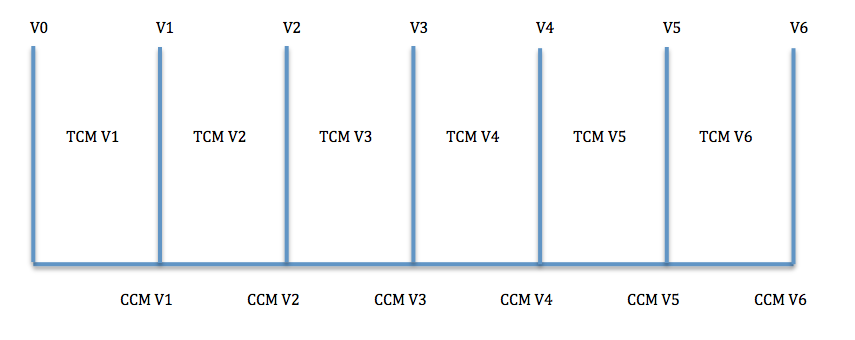
\includegraphics[width=0.5\textwidth]{change_complexity_figure}
   \caption{"Change Complexity vs. Traditional Complexity"}
   \label{fig:ccVstc}
\end{figure}



\begin{equation} \label{eq:Eq2}
{{CCM_{v(i)}} = {TCM_{v(i+1)}}-{TCM_{v(i)}}}
\end{equation}

\begin{equation} \label{eq:Eq3}
{{TCM_{v(i+1)}} = \sum\limits_{i=0}^iCCM_{v(i)}}
\end{equation}
 
\begin{equation}  \label{eq:Eq4}
{{{TCM_{v(i)}} = CCM_{v(i)}}   _{n=1000}}
\end{equation}

\section{Results and Discussion}

It has been previously shown that Halstead's length, volume, level and mental discriminations all correlate highly with each other \cite{Israel}, so it is safe to select hlen only of these metrics. Maxcy and sloc have also shown to correlate highly with each other so Maxcy has been chosen. Total cyclomatic complexity has been also added as it provides the complexity measure for the sum of all functions. Finally, loc has been included as it is a measure of all text lines in the code. For measures pertaining to change complexity, we have chosen the simplest ones that adequately capture change complexity. 
\newline

{\bf{\emph Q1) Does the difference of traditional complexity measures before and after a change correlate with change complexity measures?}}
\newline

We measure the difference between traditional complexity measures before and after a change and relate that with the change complexity measure at that particular change. By examining the result, we can see that measures that are related to change complexity correlate very poorly with those of system complexity (\textless 0.3).
\newline

\begin{table}[ht]

\centering
\resizebox{8cm}{!}{
\begin{tabular}{r||rrrrrrr}
  \hline
 & mods & hunk\_dist & indent\_sum & loc & hlen & maxcy & totcy \\ 
  \hline
mods & 1.00 & 0.65 & 0.85 & 0.30 & 0.26 & 0.23 & 0.26 \\ 
  hunk\_dist & 0.65 & 1.00 & 0.63 & 0.18 & 0.16 & 0.11 & 0.14 \\ 
  indent\_sum & 0.85 & 0.63 & 1.00 & 0.28 & 0.24 & 0.22 & 0.24 \\ 
  loc & 0.30 & 0.18 & 0.28 & 1.00 & 0.89 & 0.54 & 0.73 \\ 
  hlen & 0.26 & 0.16 & 0.24 & 0.89 & 1.00 & 0.51 & 0.70 \\ 
  maxcy & 0.23 & 0.11 & 0.22 & 0.54 & 0.51 & 1.00 & 0.64 \\ 
  totcy & 0.26 & 0.14 & 0.24 & 0.73 & 0.70 & 0.64 & 1.00 \\ 
   \hline
\end{tabular}}
\caption {\small Correlation Matrix of Research Question 1.}
\label{tab:table1} 

\end{table}

{\bf{\emph Q2)Does the weighted sum of change complexity measures up to a version correlated with the traditional complexity measures at that version? }}
\newline

We measured the last 1000 commits' weighted sum of change complexity measures up to a single version and compared it with the traditional complexity measures of that version. By looking at the results in table \ref{tab:table2}, we can see that change complexity measures correlated negatively with traditional complexity measures.
\newline

\begin{table}[ht]
\centering
\resizebox{8cm}{!}{
\begin{tabular}{r||rrrrrrr}
  \hline
 & mods & hunk\_dist & indent\_sum & loc & hlen & maxcy & totcy \\ 
  \hline
mods & 1.00 & 0.25 & 0.96 & -0.23 & -0.21 & -0.38 & -0.36 \\ 
  hunk\_dist & 0.25 & 1.00 & 0.31 & -0.21 & -0.22 & -0.19 & -0.20 \\ 
  indent\_sum & 0.96 & 0.31 & 1.00 & -0.18 & -0.16 & -0.32 & -0.30 \\ 
  loc & -0.23 & -0.21 & -0.18 & 1.00 & 1.00 & 0.95 & 0.96 \\ 
  hlen & -0.21 & -0.22 & -0.16 & 1.00 & 1.00 & 0.94 & 0.95 \\ 
  maxcy & -0.38 & -0.19 & -0.32 & 0.95 & 0.94 & 1.00 & 1.00 \\ 
  totcy & -0.36 & -0.20 & -0.30 & 0.96 & 0.95 & 1.00 & 1.00 \\ 
   \hline
\end{tabular}}
\caption {\small Correlation Matrix of Research Question 2.}
\label{tab:table2} 
\end{table}


{\bf{\emph Q3)Do the traditional measures calculated on only the files that had changed at a certain commit correlate with the change complexity measures at the last 1000 changes?}}
\newline

To answer the third research question, first we identified the files that have undergone changes in a version and extracted the traditional measures for them. Then, we measured the change complexity measures for the last 1000 changes and compared these two measures.  Table \ref{tab:table3} shows the correlation matrix which shows that there is a very poor correlation between the change complexity measures and traditional complexity measures (\textless 0.3).

\begin{table}[ht]

\centering
\resizebox{8cm}{!}{
\begin{tabular}{r||rrrrrrr}
  \hline
 & mods & hunk\_dist & indent\_sum & loc & hlen & maxcy & totcy \\ 
  \hline
mods & 1.00 & 0.66 & 0.86 & 0.23 & 0.23 & 0.21 & 0.23 \\ 
  hunk\_dist & 0.66 & 1.00 & 0.63 & 0.27 & 0.26 & 0.22 & 0.28 \\ 
  indent\_sum & 0.86 & 0.63 & 1.00 & 0.26 & 0.26 & 0.28 & 0.27 \\ 
  loc & 0.23 & 0.27 & 0.26 & 1.00 & 0.99 & 0.82 & 0.96 \\ 
  hlen & 0.23 & 0.26 & 0.26 & 0.99 & 1.00 & 0.85 & 0.96 \\ 
  maxcy & 0.21 & 0.22 & 0.28 & 0.82 & 0.85 & 1.00 & 0.84 \\ 
  totcy & 0.23 & 0.28 & 0.27 & 0.96 & 0.96 & 0.84 & 1.00 \\ 
   \hline
\end{tabular}}
\caption {\small Correlation Matrix of Research Question 3.}
\label{tab:table3} 
\end{table}

From the previous results of each of our research questions, we can see that syntactic complexity metrics don't provide more complexity information than lines of code do. We have also identified that traditional and change complexity measures correlate very poorly. This is due to the nature of how these measurements are extracted and what they concretely measure. For example, change complexity measures are extracted from diffs, revisions and patches as opposed to traditional complexity measures, which are extracted from the source code as a whole \cite{Hindle}. We can therefor explain the poor correlation with the underlying artifacts that these metrics are based on. Therefor, these complexity measures can not be substituted to be used as a proxy for the amount of effort that is needed to comprehend a piece of code. \newline
A snapshot of the project from it's start date until it's end date is shown in the next figures. The traditional complexity measures is shown in Figure \ref{fig:tct} in isolation, namely Locs, Totcy and Hlen. We can see that they all follow an increasing trend with Hlen and Loc decreasing at the same points in time.\newline
The change complexity measures (Mods, Hunk dist and Indent Sum) is shown in Figure \ref{fig:cct} also in isolation. They too follow a same trend with respect to each other. Finally, figure \ref{fig:TandCCT} shows the totCy and Hunk dist. In this case, we can see that they follow very different trends. This confirms that these two metrics indeed measure different things.





%Traditional Complexity timeseries
\begin{figure}[h!]
  \centering
  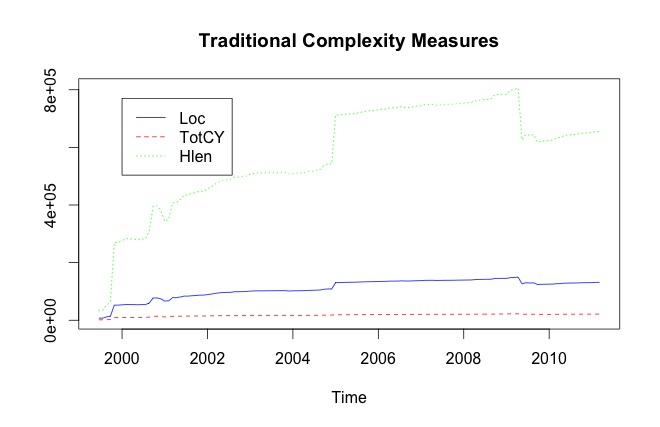
\includegraphics[width=0.5\textwidth]
  {TradPlot}
   \caption{Traditional Complexity Measures Timeseries }
   \label{fig:tct}
\end{figure}

%Change Complexity timeseries
\begin{figure}[h!]
  \centering
  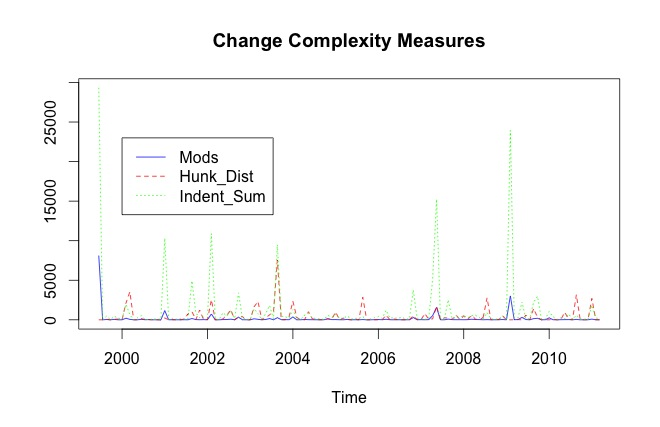
\includegraphics[width=0.5\textwidth]
  {ChangePlot}
   \caption{Change Complexity Measures Timeseries }
   \label{fig:cct}
\end{figure}

%Change and Traditional Complexity timeseries
\begin{figure}[h!]
  \centering
  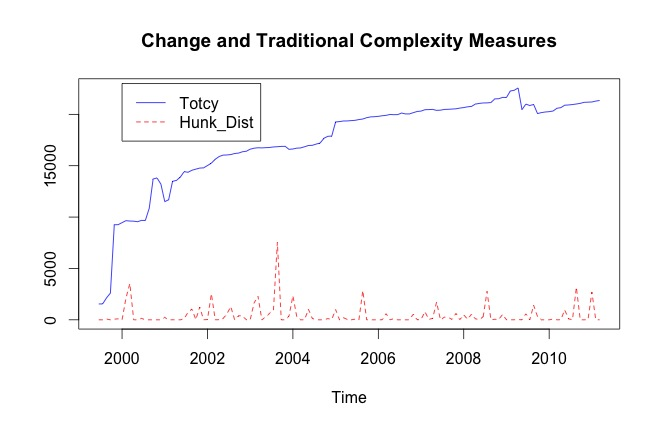
\includegraphics[width=0.5\textwidth]{ChangeandTradPlot}
   \caption{Traditional and Change Complexity Measures Timeseries }
   \label{fig:TandCCT}
\end{figure}

\section{Threats to Validity}
In our study we calculated the complexity measures on each particular commits (aka. each version), however the correlation between traditional complexity measures in Israel's study \cite{Israel} was done at a file level. Israel also made account of the confounding effect of file size. The result was that even though file size influences the values of the correlations, it does not substantially change the conclusion extracted from those correlations in any case. Therefor, in order to rule out this effect, the total size of the system must be taken into consideration. Another threat to validity is the source of inconsistencies in measuring traditional complexity metrics between header files and non-header files.
\section{Conclusion}

In this work we have chosen the Apache HTTP Server Open Source Project and extracted data related to traditional and change complexity measures within a 12-year period. For each of our research questions, we have shown that
traditional complexity measures, in particular those that are exclusively based on the structure of the program or properties of text, do not provide additional information on the amount of effort that's required to fully understand a piece of code. Therefor, lines of code are sufficient to comprehend code fragments. We have also shown that, for each research question, while change complexity measures correlate very strongly with one another, the same result is not the case with traditional complexity measures (in some cases, there is a negative relationship). This is because they measure different things in different contexts and therefor results in a weak relationship between them.



\section{Future Work}
Future research directions include using traditional and change complexity metrics as an indication of the maintainability and evolvability of a system; such as productivity and number of bugs.

\begin{thebibliography}{9}

\bibitem{Israel}
I. Herraiz, A. Hassan  {\em Beyond Lines of Code: Do We Need More Complexity Metrics?} Making Software. Greg Wilson and Andy Oram,
  O'Reilly Media, Inc., 
  2010.
  
\bibitem{Peter}
P. Rigby (2011), {\em Understanding Open Source Software Peer Review:
Review Processes, Parameters and Statistical Models, and
Underlying Behaviours and Mechanisms.},  
Ph.D. Thesis. University of Victoria, Canada.

\bibitem{Hindle}
A. Hindle, M. W. Godfrey, R. C. Holt. {\em Reading Beside the Lines: Indentation as a Proxy for Complexity Metrics.} In ICPC: Proceedings of the 16th IEEE International
Conference on Program Comprehension, pages 133-142. IEEE Computer Society,
2008.


\bibitem{Graves}
T. L. Graves, A. F. Karr, J. S. Marron, and H. Siy. {\em Predicting fault incidence using
software change history.} IEEE Trans. Softw. Eng., 26(7):653-661, 2000.

\bibitem{Leszak}
M. Leszak, D. E. Perry, and D. Stoll. { \em Classification and evaluation of defects in a
project retrospective.} Journal of Systems and Software, 61(3):173-187, 2002.

\bibitem{Herraiz}
I. Herraiz, J. M. Gonzalez-Barahona, and G. Robles. { \em Towards a theoretical model
for software growth.} In MSR: Proceedings of the Fourth International Workshop on
Mining Software Repositories, pages 21-28. IEEE Computer Society, 2007.




\end{thebibliography}
\end{document}
